\documentclass[a4paper, 11pt]{article}           %{{{1
% basic packages                                 {{{2
\usepackage[T1]{fontenc}
\usepackage[scaled=0.975]{helvet}
\usepackage[utf8]{inputenc}
\usepackage{amsmath}
\usepackage{lastpage}
\usepackage{graphicx}
\usepackage{tcolorbox}                                                          % encadrement texte
\usepackage{xcolor}
\usepackage{listings}                                                           %
\usepackage{multicol}
% listings                                        {{{3
\definecolor{mygreen}{rgb}{0,0.6,0}
\definecolor{mygray}{rgb}{0.5,0.5,0.5}
\definecolor{mymauve}{rgb}{0.58,0,0.82}
\definecolor{deepblue}{rgb}{0,0,0.5}
\definecolor{deepred}{rgb}{0.6,0,0}
\definecolor{deepgreen}{rgb}{0,0.5,0}
\lstset{%
%       backgroundcolor=\color{white},   % choose the background color; you must add \usepackage{color} or \usepackage{xcolor}; should come as last argument
%       basicstyle=\footnotesize,        % the size of the fonts that are used for the code
%       breakatwhitespace=false,         % sets if automatic breaks should only happen at whitespace
%       breaklines=true,                 % sets automatic line breaking
%       captionpos=b,                    % sets the caption-position to bottom
        commentstyle=\color{mygreen},    % comment style
%       deletekeywords={type},           % if you want to delete keywords from the given language
%       emph={},                         % Custom highlighting
%       emphstyle=\ttb\color{deepred}    % Custom highlighting style
%       escapeinside={\%*}{*)},          % if you want to add LaTeX within your code
%       extendedchars=true,              % lets you use non-ASCII characters; for 8-bits encodings only, does not work with UTF-8
        frame=shadowbox,                 % adds a frame around the code {single, shadowbox}
%       keepspaces=true,                 % keeps spaces in text, useful for keeping indentation of code (possibly needs columns=flexible)
        keywordstyle=\color{blue},       % keyword style
	language=C,                      % the language of the code {Python, C}
%       morekeywords={*,...},            % if you want to add more keywords to the set
        numbers=left,                    % numbers = (none, left, right)
%       numbersep=5pt,                   % how far the line-numbers are from the code
%       numberstyle=\tiny\color{mygray}, % the style that is used for the line-numbers
%       otherkeywords={self},            % Add keywords here
%       rulecolor=\color{black},         % if not set, the frame-color may be changed on line-breaks within not-black text (e.g. comments (green here))
	rulesepcolor=\color{gray}        % shadowbox color
%       showspaces=false,                % show spaces everywhere adding particular underscores; it overrides 'showstringspaces'
%       showstringspaces=false,          % underline spaces within strings only
%       showtabs=false,                  % show tabs within strings adding particular underscores
%       stepnumber=1,                    % the step between two line-numbers. If it's 1, each line will be numbered
%       stringstyle=\color{mymauve},     % string literal style
%       tabsize=4,                       % sets default tabsize to 2 spaces
%       title=\lstname                   % show the filename of files included with \lstinputlisting; also try caption instead of title
}
%}}}
%}}}
% mise en page                                   {{{2
\addtolength{\voffset}{-1.8cm}
\addtolength{\textheight}{4cm}
\addtolength{\hoffset}{-2.5cm}
\addtolength{\textwidth}{4cm}
\addtolength{\headsep}{-0.5cm}
\usepackage{fancyhdr}
\setlength{\headheight}{14.00pt}
\pagestyle{fancy} % Numérotation des pages
\renewcommand\headrulewidth{1pt}
\renewcommand\footrulewidth{1pt}
\fancyhead[L]{BP SN}
\fancyhead[C]{arduino}
\fancyhead[R]{automatique, moteur, capteur, CAN}
\fancyfoot[L]{v 1.3}
\fancyfoot[C]{\textbf{gestion de l'habitat : air}}
\fancyfoot[R]{\thepage/\pageref{LastPage}}
%}}}
% Compteurs:                                     {{{2
\addtocounter{page}{0}
\newcounter{Q}
\newcounter{exoNB}
%}}}
% Longueur:                                      {{{2
\newlength{\longueurA}
\newlength{\longueurB}
\setlength{\parindent}{0pt}
\setlength{\parskip}{2pt}
\renewcommand{\baselinestretch}{1}
%}}}
% newcommand                                     {{{2
\newcommand{\question}{\stepcounter{Q} $\boxed{\arabic{Q}}$ }
\newcommand{\reponse}{
\par\nobreak
\noindent\rule{0pt}{1.5\baselineskip}% Provides a larger gap between the preceding paragraph and the dots
{\noindent\makebox[\linewidth]{\dotfill}\endgraf}% ... dotted lines ...
% \bigskip% Gap between dots and next paragraph
}
\newcommand{\ligne}{\underline{\hspace{ \textwidth}} }
\newcommand{\exo}[1]{\stepcounter{exoNB}\textsc{\Large Exercice \arabic{exoNB} -- #1} }
\newcommand{\EXO}[2]{\stepcounter{exoNB}\textsc{\Large Exercice \arabic{exoNB} -- #1} \hfill \textbf{#2 points}}
\newcommand{\pb}[1] {\stepcounter{exoNB}\textsc{\Large Problème \arabic{exoNB} -- #1} }
\newcommand{\PB}[2] {\stepcounter{exoNB}\textsc{\Large Problème \arabic{exoNB} -- #1} \hfill \textbf{#2 points}}

\newcommand{\objectif}[1]{\textsc{\huge \textbf{Objectif :}\\[2mm] #1} }
\newcommand{\partie}[1]{\textsc{\Large #1} }
%}}}
% Divers                                         {{{2
% PRL style line                                 {{{3
\newlength{\diamondrulelength}
\setlength{\diamondrulelength}{0.6\textwidth}
\newlength{\diamondrulethickness}
\setlength{\diamondrulethickness}{2pt}
\newcommand{\diamondrule}{\begin{center}\tikz{\fill[black] (0.5\diamondrulelength,0) -- (0,0.5\diamondrulethickness) -- (-0.5\diamondrulelength,0) -- (0,-0.5\diamondrulethickness) -- cycle;}\end{center}}
%}}}
% fixed with tabular                             {{{3
\usepackage{array}
\newcolumntype{L}[1]{>{\raggedright\let\newline\\\arraybackslash\hspace{0pt}}m{#1}}
\newcolumntype{C}[1]{>{\centering\let\newline\\\arraybackslash\hspace{0pt}}m{#1}}
\newcolumntype{R}[1]{>{\raggedleft\let\newline\\\arraybackslash\hspace{0pt}}m{#1}}
%}}}
%}}}
%}}}


% http://wiki.keyestudio.com/index.php/Ks0080(81,_82)keyestudio_Maker_Learning_Kit_for_Arduino#Project_5:_Traffic_Light

\begin{document}
\sffamily
\hfill Nom : {\noindent\makebox[5cm]{\dotfill}\endgraf}
\objectif{Alimenter un moteur par un transistor et le contrôler automatiquement.}

Ce sujet va vous apprendre à alimenter un moteur par une alimentation séparée de l'électronique de commande, ici et comme souvent le microcontrolleur. De plus, nous allons programmer ce microcontrolleur pour commander le moteur en fonction d'une mesure de la température. L'idée est que nous allons ventiller quand il fait chaud.

\bigskip

\partie{Materiel} \\                      %{{{1
Pour le montage du moteur alimenté par un transistor :
\begin{multicols}{2}
- Arduino Board *1 \\
- USB Cable *1 \\
- TIP122 Triode*1  \\
- 9V Battery *1  \\
- 1 K$\Omega$ Resistor *1 \\
- Fan Motor *1 \\
- Fan Leaf *1 \\
- Bread Board *1 \\
- Breadboard Jumper Wires \\
- \emph{LM35 Temperature Sensor *1}
\end{multicols}

%}}}

\bigskip

\partie{Cablage d'un moteur par un transistor bipolaire.}\\             %{{{1
\begin{figure}[!b]
\begin{center}
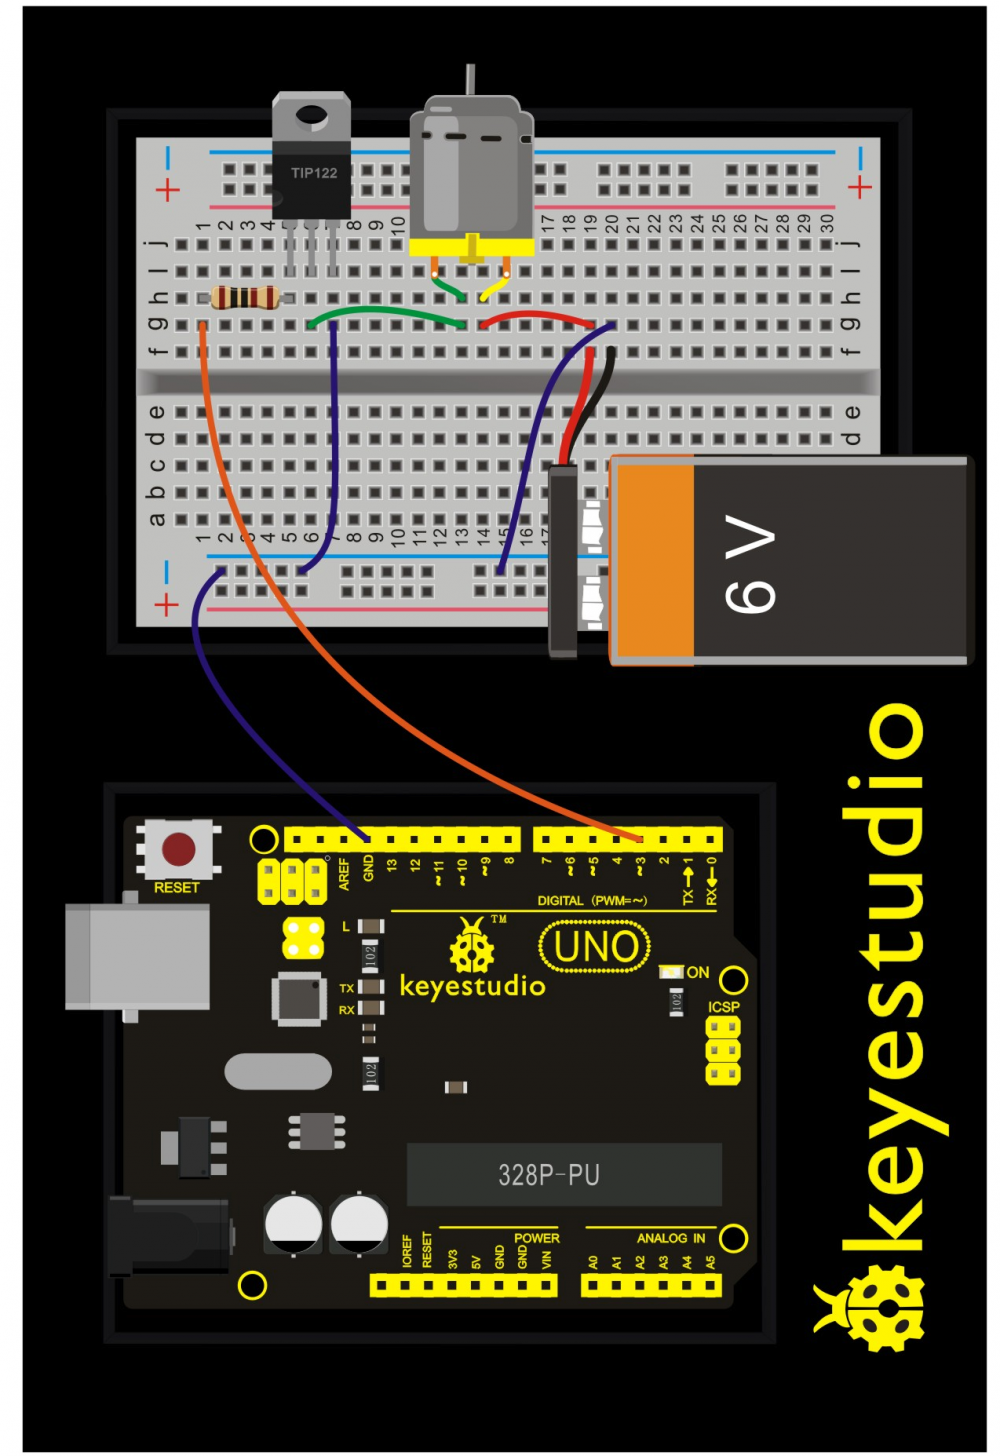
\includegraphics[height=\textwidth, angle=270]{cablage_moteur}
\caption{Alimentation du moteur par un transistor bipolaire.}
\label{CablageMoteur}
\end{center}
\end{figure}

Comme nous allons le voir, le moteur ne peut pas être directement alimenté par le microcontrolleur. Nous allons donc utiliser un transistor fonctionnant en mode interrupteur. Nous aurions pu utiliser utiliser un relais. L'alimentation sera fournie par une batterie externe de quelques volts. Si des batteries ne sont pas disponibles, nous brancherons le moteur sur la sortie 3.3V du microcontrolleur et nous risquerons de griller soit le regulateur 3.3V de la carte, soit le port USB qui alimente toute la carte en 5V, dont le regulateur 3.3V qui fournit donc les 3.3V. En fait, il y a des chances que le regulateur soit protégé en température : il s'éteind quand il est trop chaud. Il y aussi des chances que le port USB de l'ordinateur se coupe si des courants trop importants sont demandés.

\question Quel est le courant maximal que peut délivrer une sortie  ATMEGA328 de la carte UNO ?
\reponse

\question Quel est le courant maximal que peut supporter ce transistor TIP122, d'après la datasheet que vous pouvez trouver sur internet ?
\reponse

\question Lire la datasheet du regulateur de la carte UNO et spécifier d'une part son courant de sortie maximal, et d'atre part son mode de protection.
\reponse
\reponse

\question Trouver le courant maximal que peut débiter le port USB de votre ordinateur et préciser son mode de protection
\reponse

\question Réalisez le cablage de la figure \ref{CablageMoteur}, avec l'hélice sur le moteur. Alimentez le transistor et donc le moteur comme décrit en introduction à cette partie.

\question Impémenter le code suivant et faites constater au professeur.
\begin{lstlisting}
// the setup function runs once when you press reset or power the board
void setup() {
  // initialize digital pin 3 as an output.
  pinMode(3, OUTPUT);
}

// the loop function runs over and over again forever
void loop() {
  digitalWrite(3, HIGH); // turn the motor on (HIGH is the voltage level)
  delay(2000);           // wait for 2 seconds
  digitalWrite(3, LOW);  // turn the motor off by making the voltage LOW
  delay(3000);           // wait for 3 second
}
\end{lstlisting}

\tcbox{\textbf{Constatation professeur :} \hspace{5cm} } % package tcolorbox

\question Décrire l'algorithme.
\reponse

\question Dans un moteur à courant continu, quelle relation simple lie la force contre-électromotrice et la vitesse de rotation ? \footnote{voir wikipedia par exemple}
\reponse

\question Dans un moteur à courant continu, quelle relation simple lie le courant et le couple ?
\reponse

\question Dans un moteur à courant continu, en gros, quelle est la relation entre  la vitesse de rotation et la tension ?
\reponse

\question Maintenant, plus exactement, quelle est la relation qui lie la tension appliquée au courant, à la résistance du moteur et la force contre-électromotrice ?\footnote{voir wikipedia par exemple}
\reponse

\question Si l'hélice devient plus grande, comment varie le courant à vitesse de rotation constante ?
\reponse

\question Si l'hélice devient plus grande, comment varie la tension à courant constant ?
\reponse

\question A couple constant, comment faire accélérer la vitesse de rotation ?
\reponse

\question A tension appliquée constante, comment faire accélérer la vitesse de rotation ?
\reponse

\smallskip

\question Le transistor n'est pas en régime d'amplification. Ici, quel est le nom donné à son régime de fonctionnement ? Pouvez vous élaborer un peu sur ces deux régimes de fonctionnement.
\reponse
\reponse
\reponse


%}}}

\bigskip

\partie{Capteur de température}\\ %{{{1

\begin{figure}[h!]
\begin{center}
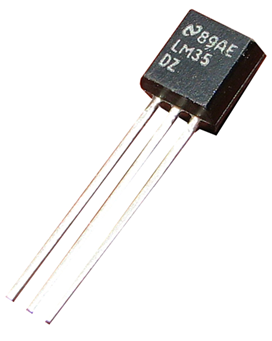
\includegraphics[width=0.15\textwidth]{LM35}
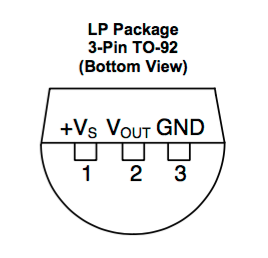
\includegraphics[width=0.25\textwidth]{LM35pinout}
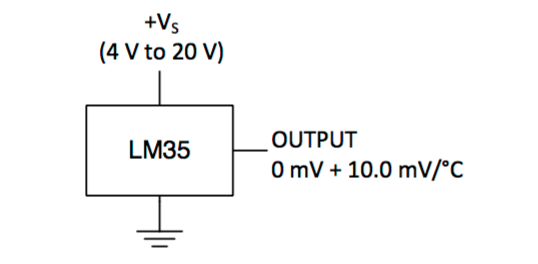
\includegraphics[width=0.55\textwidth]{LM35application}
\caption{LM35 ; voir \texttt{http://www.ti.com/lit/ds/symlink/lm35.pdf}}
\label{LM35}
\end{center}
\end{figure}
%
\question Implémentez le code ci-dessous. Donnez les deux valeurs (stabilisées) de la température lue sur le terminal série du logiciel arduino. Une mesure est faite en mettant votre doigt sur le capteur et l'autre en laissant le capteur à l'air ambiant.
\reponse
\reponse

\begin{lstlisting}
void setup() {
  Serial.begin(9600);
}
void loop() {
  // read temperature value of LM35
  int vol = analogRead(A0) * (5.0 / 1024.0*100);

  Serial.print("Tep:");
  Serial.print(vol);
  Serial.println("C");

  if (vol<22) {
    Serial.println("Froid");
  }
  else (vol>=22 ) {
    Serial.println("Chaud");
  }
}
\end{lstlisting}

\question Quelle valeur choissisez vous aux lignes 12 et 16 pour que la detection entre le chaud et le froid soit convaincante.
\reponse

\medskip

\tcbox{\textbf{Constatation professeur :} \hspace{5cm} } % package tcolorbox

\question Implémentez le code ci-dessous et donnez la valeur lue.
\reponse
\begin{lstlisting}
void setup() {
  Serial.begin(9600);
}
void loop() {
  int vol = analogRead(A0);
  Serial.print(vol);
}
\end{lstlisting}

\question Branchez l'entrée analogique A0 à la masse de la carte et donnez la valeur lue par le microcontrolleur, dont le principe de conversion est indiqué dans la figure \ref{CAN}.
\reponse

\begin{figure}[!ht] % [!h] [ht] ! pour forcer, ht Here ou Top sinon page indépendante
\centering
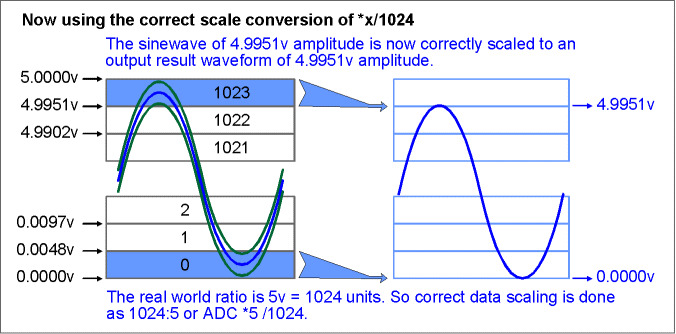
\includegraphics[width=\textwidth]{CAN}
\caption{Principe de la conversion analogique numérique. Un signal est analogique, et l'autre est numérique.}
\label{CAN} %\ref{fig_test}
\end{figure}

\question Branchez l'entrée analogique A0 au 5V de la carte donnez la valeur lue.
\reponse

\question Implémentez le code ci-dessous et donnez les deux valeurs lues en branchant l'entrée A0 à 0V et à 5V.
\reponse

\begin{lstlisting}
void setup() {
  Serial.begin(9600);
}
void loop() {
  int vol = analogRead(A0) /1024.0;
  Serial.print(vol);
}
\end{lstlisting}

\question Implémentez le code ci-dessous et donnez les deux valeurs lues en branchant l'entrée A0 à 0V et à 5V.
\reponse
\begin{lstlisting}
void setup() {
  Serial.begin(9600);
}
void loop() {
  int vol = analogRead(A0) * 5 / 1024.0;
  Serial.print(vol);
}
\end{lstlisting}

\question Branchez l'entrée A0 au LM35, puis donnez la valeur lue à la console série arduino. Combien mesure un voltmètre entre la masse et la broche Vout du LM35, celle qui est évidemment branchée à l'entrée A0.
\reponse

\question Dans la figure \ref{LM35}, quelle est l'augmentation en mV de la sortie Vout pour une augmentation de 1 degré celcius ?  
\reponse

\question Du coup, si l'on mesure une température de 10 mV à la sortie du LM35, quelle est la témpérature en degré celcius ?
\reponse

\question Du coup, si l'on mesure une température de 1 V à la sortie du LM35, quelle est la témpérature en degré celcius ?
\reponse

\question Du coup, à quoi sert la formule \texttt{analogRead(A0) * (5.0 / 1024.0*100);} ?
\reponse

\question Pour résumer, pour une température de 2 degrés Celcius, quelle est la sortie du LM35 ? \\
Quelle est la valeur lue par la fonction \texttt{analogRead(A0)} ? \\
Quel est la valeur de \texttt{analogRead(A0) * (5.0 / 1024.0); } ?\\
Quel est la valeur de \texttt{analogRead(A0) * (5.0 / 1024.0*100); }  ?
\reponse
\reponse
\reponse
\reponse



%}}}

\bigskip

\partie{Ventilation mécanique contrôlée}\\               %{{{1

Dans cette dernière partie, la réalisation est une ventillation qui se déclenche au dessus d'une température. Le code source n'est pas donné parce qu'il est à trouver en combinant les sources vues dans les parties précédentes.


\question Combinez les deux parties précédentes pour réaliser le code et le montage d'une ventillation contrôlée par la température. Décrivez ci-après le code source dans les grandes lignes.

\medskip
\textbf{Code source :}
\reponse
\reponse
\reponse
\reponse
\reponse
\reponse
\reponse
\reponse
%
\textbf{Montage :}
\tcbox{\textbf{Constatation professeur :} \hspace{5cm} } % package tcolorbox

%}}}

\end{document}


% vim:fdl=0
